\chapter{AdaptaMaterialEscolar 2.0}
\label{cap:AdaptaMaterialEscolar2.0}
En este capítulo explicaremos la obtención de requisitos en la Sección \ref{cap:requisitos}. También se describirá la iteración competitiva para el diseño de la aplicación en la Sección \ref{disenyoDeLaAplicacion}.

\section{Requisitos}
\label{cap:requisitos}

Lo primero que hicimos fue analizar la memoria de AdaptaMaterialEscolar 1.0 (\cite*{AdaptaMaterialEscolar1.0}) extrayendo las funcionalidades que faltaban por implementar y los resultados de la evaluación que se realizó. Tras este análisis surgieron una serie de cambios y nuevas funcionalidades. Uno de los cambios fue agrupar dichas funcionalidades en formato (funcionalidades que tienen relación con el formato de los ejercicios), en ejercicios (funcionalidades relacionadas con la realización de ejercicios) y finalmente en auxiliar (resto de funcionalidades que no pertenecen a formato o a ejercicios). Quedando las funcionalidades agrupadas de la siguiente manera:
\\

Formato: 
\begin{itemize}
  \item Añadir encabezado al texto: El usuario elijará un encabezado y se le añadirá al docuemnto.
  \item Añadir un tipo de fuente escolar: Incluir en los tipos de fuentes la escolar. Dicha fuente se refleja en la imagen \ref{escolar}.
  \begin{figure}[ht!]
    \centering
    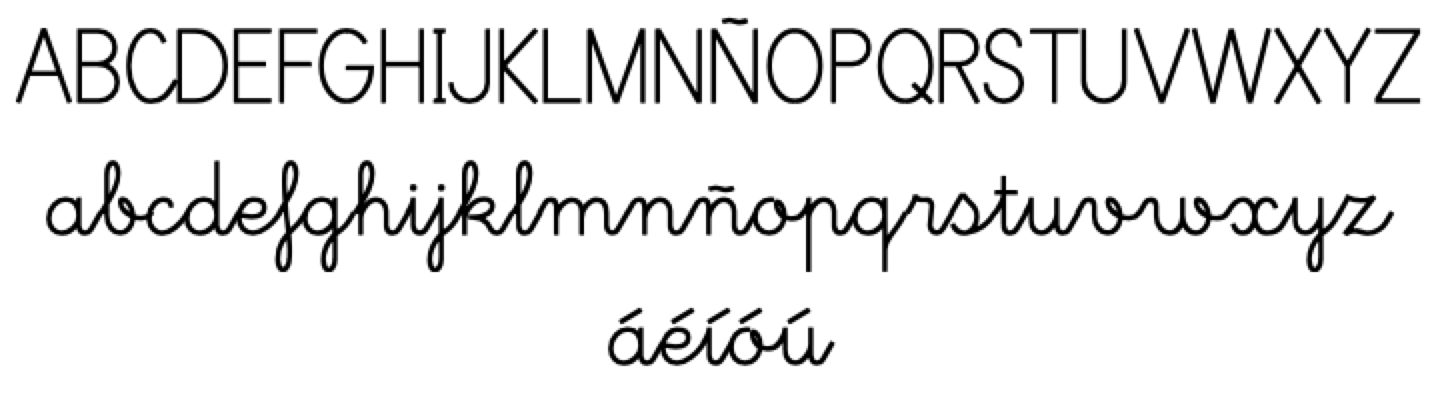
\includegraphics[scale=0.3]{AdaptaMaterialEscolar/FunteEscolar.png}
    \caption{Fuente escolar.}
    \label{escolar}
\end{figure}
  \item Añadir una leyenda de colores con la categoría de cada tipo: Crear una tabla con valores donde cada valor esta asociado a un color.
  \item Añadir leyenda de colores para el tema de cada asignatura: Dar la posibilidad de que cada asignatura tenga un color. Al crear un documento según la asignatura se pondrá el borde del documento del color que corresponde a dicha asignatura.
  \item Añadir cuadrícula para escribir los números.
  \item Añadir la alternativa de añadir doble pauta: En vez de renglones de una única línea se podrá poner para responder a una pregunta la doble pauta.
  \item Estandarizar formato para títulos e índices del temario: dar la opción de crear estilos para estandarizar documento.
  \item Enumerar ejercicios de forma automática: Establecer un orden numérico para los ejercicios de forma automática según se van creando para que el usuario no se tenga que preocupar de ese aspecto.
\end{itemize}
Ejercicios:
\begin{itemize}
  \item Ejercicios de relacionar contenido mediante flechas: Generar un ejercicio para relacionar conceptos mediante flechas.
  \item Añadir ejercicios de cálculo con huecos a rellenar por el alumno: Posibilidad de introducir ejercicios de cálculo con espacios en blanco para que el alumno rellene dichos huecos con contenido adecuado.
  \item Añadir ejercicios con espacio para dibujar: Amplio hueco en blanco con el fin de que el alumno pueda dibujar.
  \item Ejercicios de completar los espacios en blanco en tablas y esquemas: Dada una tabla o un esquema se establecen espacios en blanco para que el alumno los rellene con el contenido adecuado.
\end{itemize}
Auxiliar:
\begin{itemize}
  \item Generar un resumen a partir de un texto.
  \item Exportar el documento a formato Word.
  \item Añadir un pictotraductor: Dado una frase traducirla a pictogramas.
  \item Añadir imágenes buscando una palabra: A partir de una palabra se busca su respectiva imagen en las bases de datos de imágenes libres. Por ejemplo, con el fin de incluir en el docuemnto una imagenn para una explicación más visual .
  \item Sustituir una palabra por una imagen: Una palabra se reemplazará por una imagen.
  \item Crear una herramienta de recorte de imágenes para el texto original: habrá un botón que tras darle te permita seleccionar un área para convertirla en una imagen.
  \item Crear tablas que organicen el temario y/o las actividades, seleccionando contenido: Tras la selección de contenido por parte del usuario se creará una tabla o un esquema en base a la información seleccionada, con un formato predefinido.
  \item Creación de esquemas.
\end{itemize}
Tras haber analizado en detalle las funcionalidades anteriores hemos encontrado que varias funciones ya están implementadas en la versión original de AdaptaMaterialEscolar y otras hemos decidido no implementarlas ya que consideramos que no tenemos la información suficiente para implementarlas. Las siguientes funcionalidades son las que ya están implementadas en la versión original:
  \begin{itemize}
    \item Añadir encabezado al texto: El docuemnto editable tiene una opción para añadir un ecabezado, cuando se pulsa dicha opción el documento editable convierte el formato de la letra en el del encabezado seleccionado. 
    \item Enumerar ejercicios de forma automática: El docuemnto editable tiene dicha acción, cuando pulsas el botón para enumerar se añadirá una indexación.
  \end{itemize}
Las funcionalidades que hemos decidido descartar de momento por falta de información son las siguientes:
\begin{itemize}
  \item Añadir imágenes buscando una palabra. Partimos de que debemos usar una base de datos de imagen libre pero no tenemos la información suficiente para definir cual sería la base de datos correcta.
  \item Sustituir una palabra por una imagen: Una palabra se reemplazará por una imagen.
  \item Crear una herramienta de recorte de imágenes para el texto original: Añadir una herramienta que recorte imágenes del texto original.
  \item Crear tablas que organicen el temario y/o las actividades, seleccionando contenido: Descartamos dicha funcionalidad ya que no tenemos la información suficiente del formato que desea el usuario.
  \item Crear esquemas que faciliten la visualización: Descartamos dicha funcionalidad ya que no tenemos la información suficiente del formato que desea el usuario.
  \item Ejercicios de completar los espacios en blanco en tablas y esquemas.
\end{itemize}

Por lo tanto, las funcionalidades que vamos a implementar son las que se muestran a continuación:


\begin{itemize}
  \item Generar un resumen a partir de un texto. Se realizará con el fin de ayudar a un alumno a comprender loas elementos claves del texto de manera mas rápida.
  \item Exportar el documento a formato Word para hacer modificaciones. Se realizará para que el usuario pueda continuar con las modificiones del docuemnto. 
  \item Añadir un pictotraductor: Se realizará con el fin de trasformar un texto a pictotraductor para que el alumno pueda adquirir nuevos conocimientos de forma más sencilla.
  \item Ejercicios de relacionar contenido mediante flechas. Se realizará ya que ayuda al alumno a consolidar conceptos.
  \item Añadir un tipo de fuente escolar. Se realizará con el fin de facilitar la lectura y la escritura al alumno.
  \item Añadir una leyenda de colores con la categoría de cada tipo. Se realizará con el fin de  ayudar al alumno a relacionar conceptos. 
  \item  Añadir ejercicios de cálculo con huecos a rellenar por el alumno. Se realizará para que el alumno practique el cálculo.
  \item  Añadir ejercicios con espacio para dibujar. Se realizará con el fin de que el alumno pueda reflejar lo que piensa, interpreta y representa sobre algo.
  \item Añadir leyenda de colores para el tema de cada asignatura. Se realizará con el fin de que el alumno pueda distinguir entre las asignaturas.
  \item Añadir ejercicios de matemáticas con cuadrícula para escribir los números. Se realizará con el fin de facilitar  los ejercicios de matemáticas(NO SE)
  \item Añadir la alternativa de añadir doble pauta. Se realizará con el fin de que el alumno adquiera un tamaño de letra adecuado.
  \item Estandarizar formato para títulos e índices del temario. Con el fin de que el profesor pueda definir un estilo. 

\end{itemize}                                               

\section{Diseño de la aplicación}
\label{disenyoDeLaAplicacion}
Para el diseño de la aplicación web hemos realizado una iteración competitiva. Cada integrante del grupo ha proporcionado un diseño de las funcionalidades. El diseño de Álvaro Gómez Sittima se muestra en las figuras \ref{IteracionCompetitiva1}, \ref{IteracionCompetitiva2}, el de Dunia Namour Doughani se reflejan en la figura \ref{IteracionCompetitiva3}, el diseño de Alberto Alejandro Rivas Fernández se muestra en las figuras \ref{IteracionCompetitiva4}, \ref{IteracionCompetitivaA2}, \ref{IteracionCompetitivaA3} y por el último, el diseño de Johan Sebastian Salvatierra Gutierrez se muestra en las figuras \ref{IteracionCompetitivaJ1}, \ref{IteracionCompetitivaJ2}. Una vez que cada integrante ha explicado su diseño, hemos cogido lo mejor de cada uno. El diseño de la pantalla de inicio se muestra en la figura \ref{diseño_final}, el diseño de la funcionalidad generar un resumen a partir de un texto aparece en la figura \ref{resuemn}, el diseño de la funcionalidad añadir un pictotraductor se muestra en la figura \ref{picto}, el diseño de la funcionalidad añadir una leyenda de colores con la categoría de cada tipo se muestra en la figura \ref{leyenda}, por último, se muestra el diseño de la funcionalidad ejercicios de relacionar contenido mediante flechas en la figura \ref{flecha}. No se ha realizado diseño de todas las funcionalidades ya que algunas de ellas irán incorporadas en el editable y no en una pestaña aparte.


\begin{figure}[ht!]
    \centering
    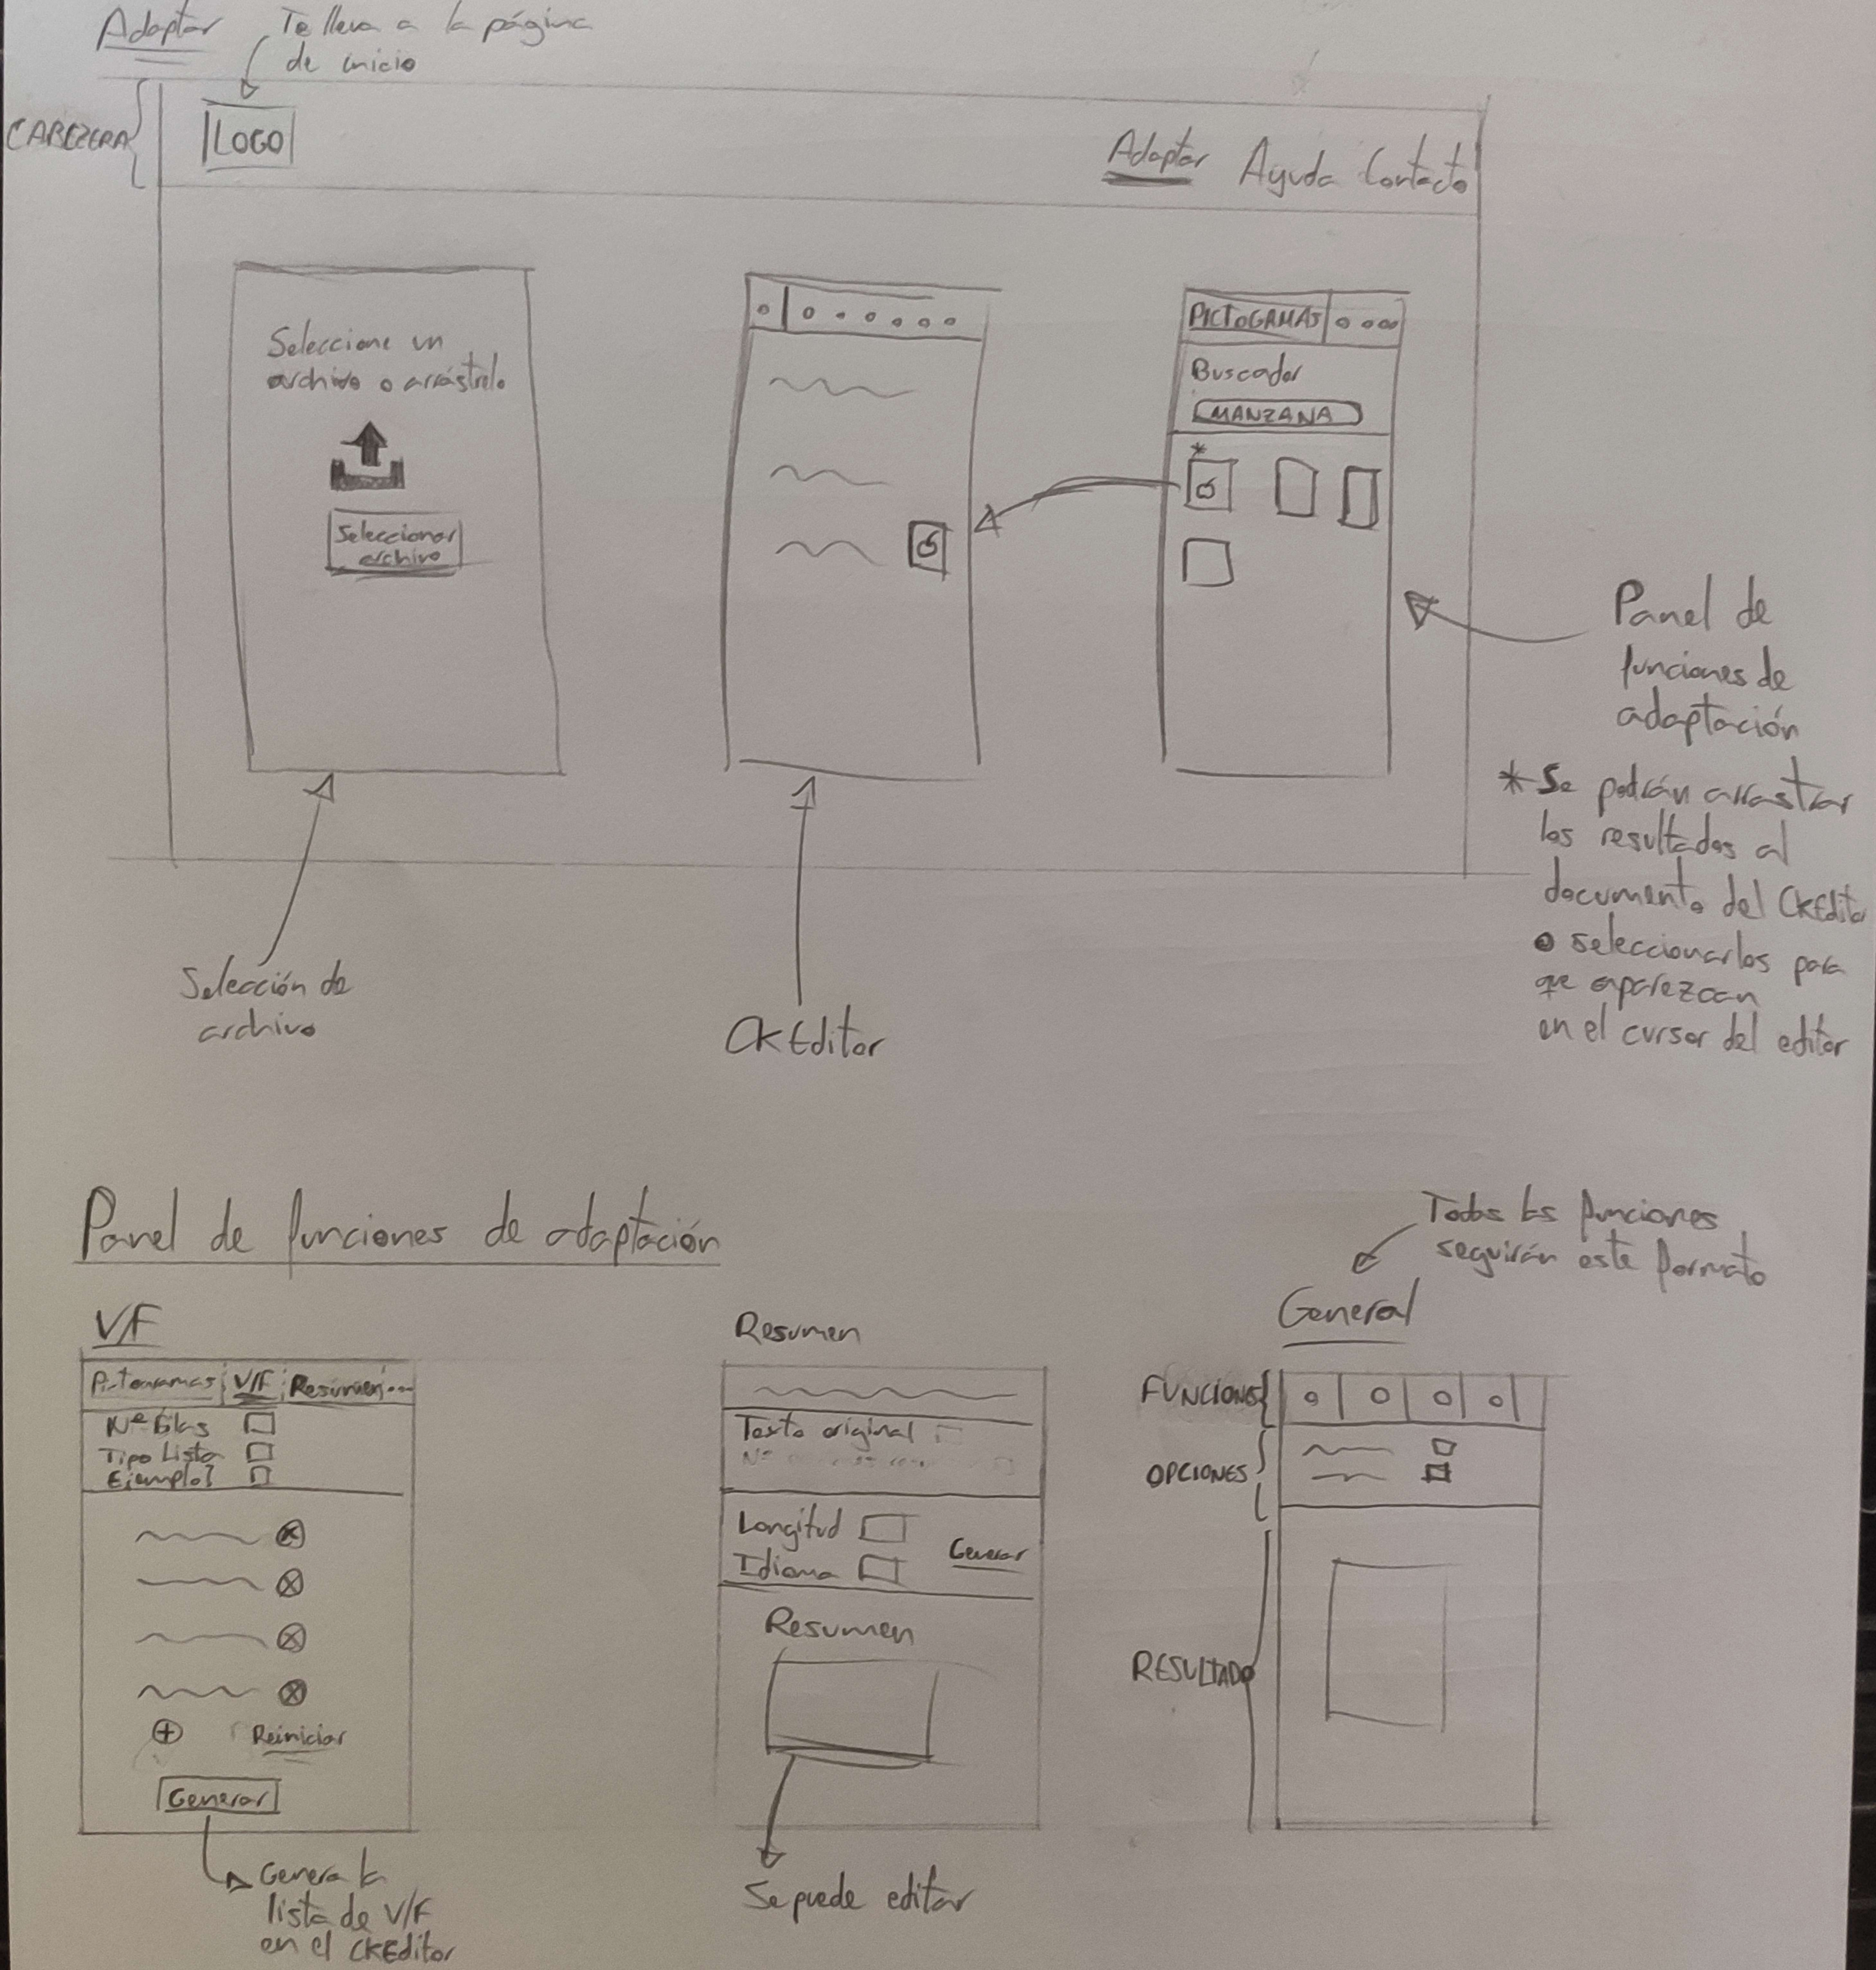
\includegraphics[width=15cm,height=16cm]{Diseño/Alvaro.jpg}
    \caption{Diseño 1 Álvaro Gómez Sittima iteración competitiva.}
    \label{IteracionCompetitiva1}
\end{figure}
\begin{figure}[ht!]
    \centering
    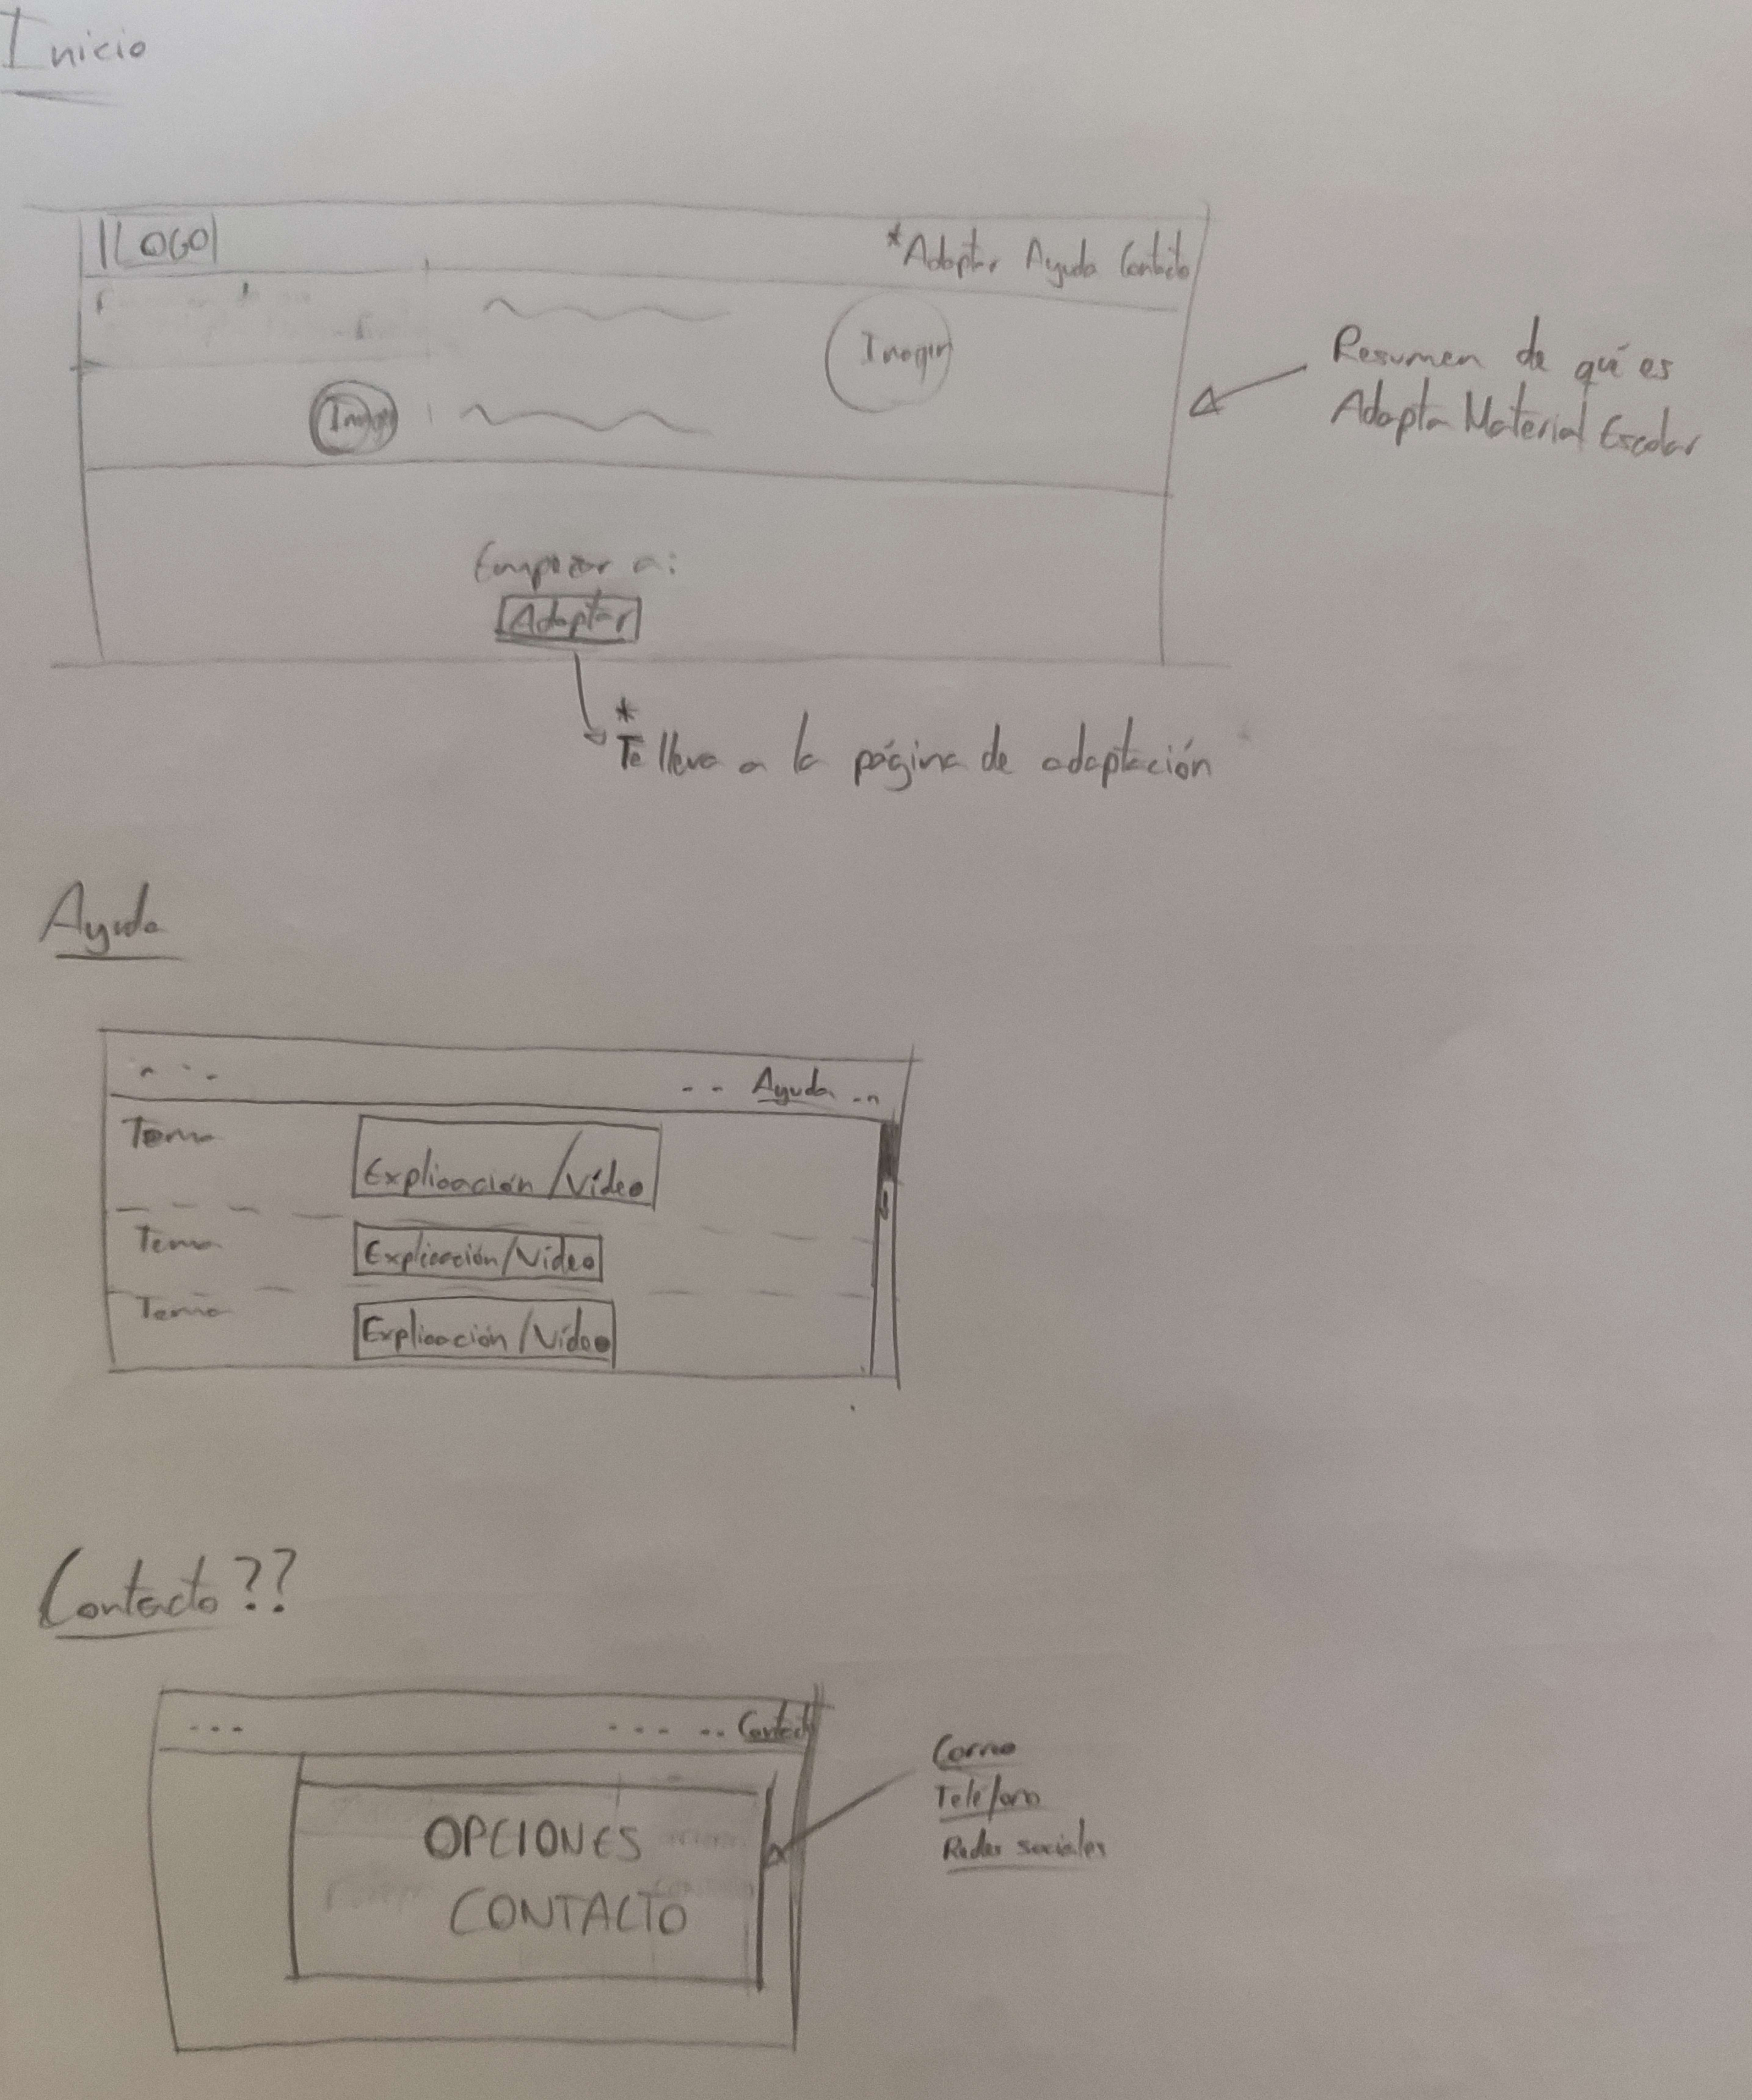
\includegraphics[width=15cm,height=16cm]{Diseño/Alvaro2.jpg}
    \caption{Diseño 2 Álvaro Gómez Sittima iteración competitiva .}
    \label{IteracionCompetitiva2}
\end{figure}
\begin{figure}[ht!]
    \centering
    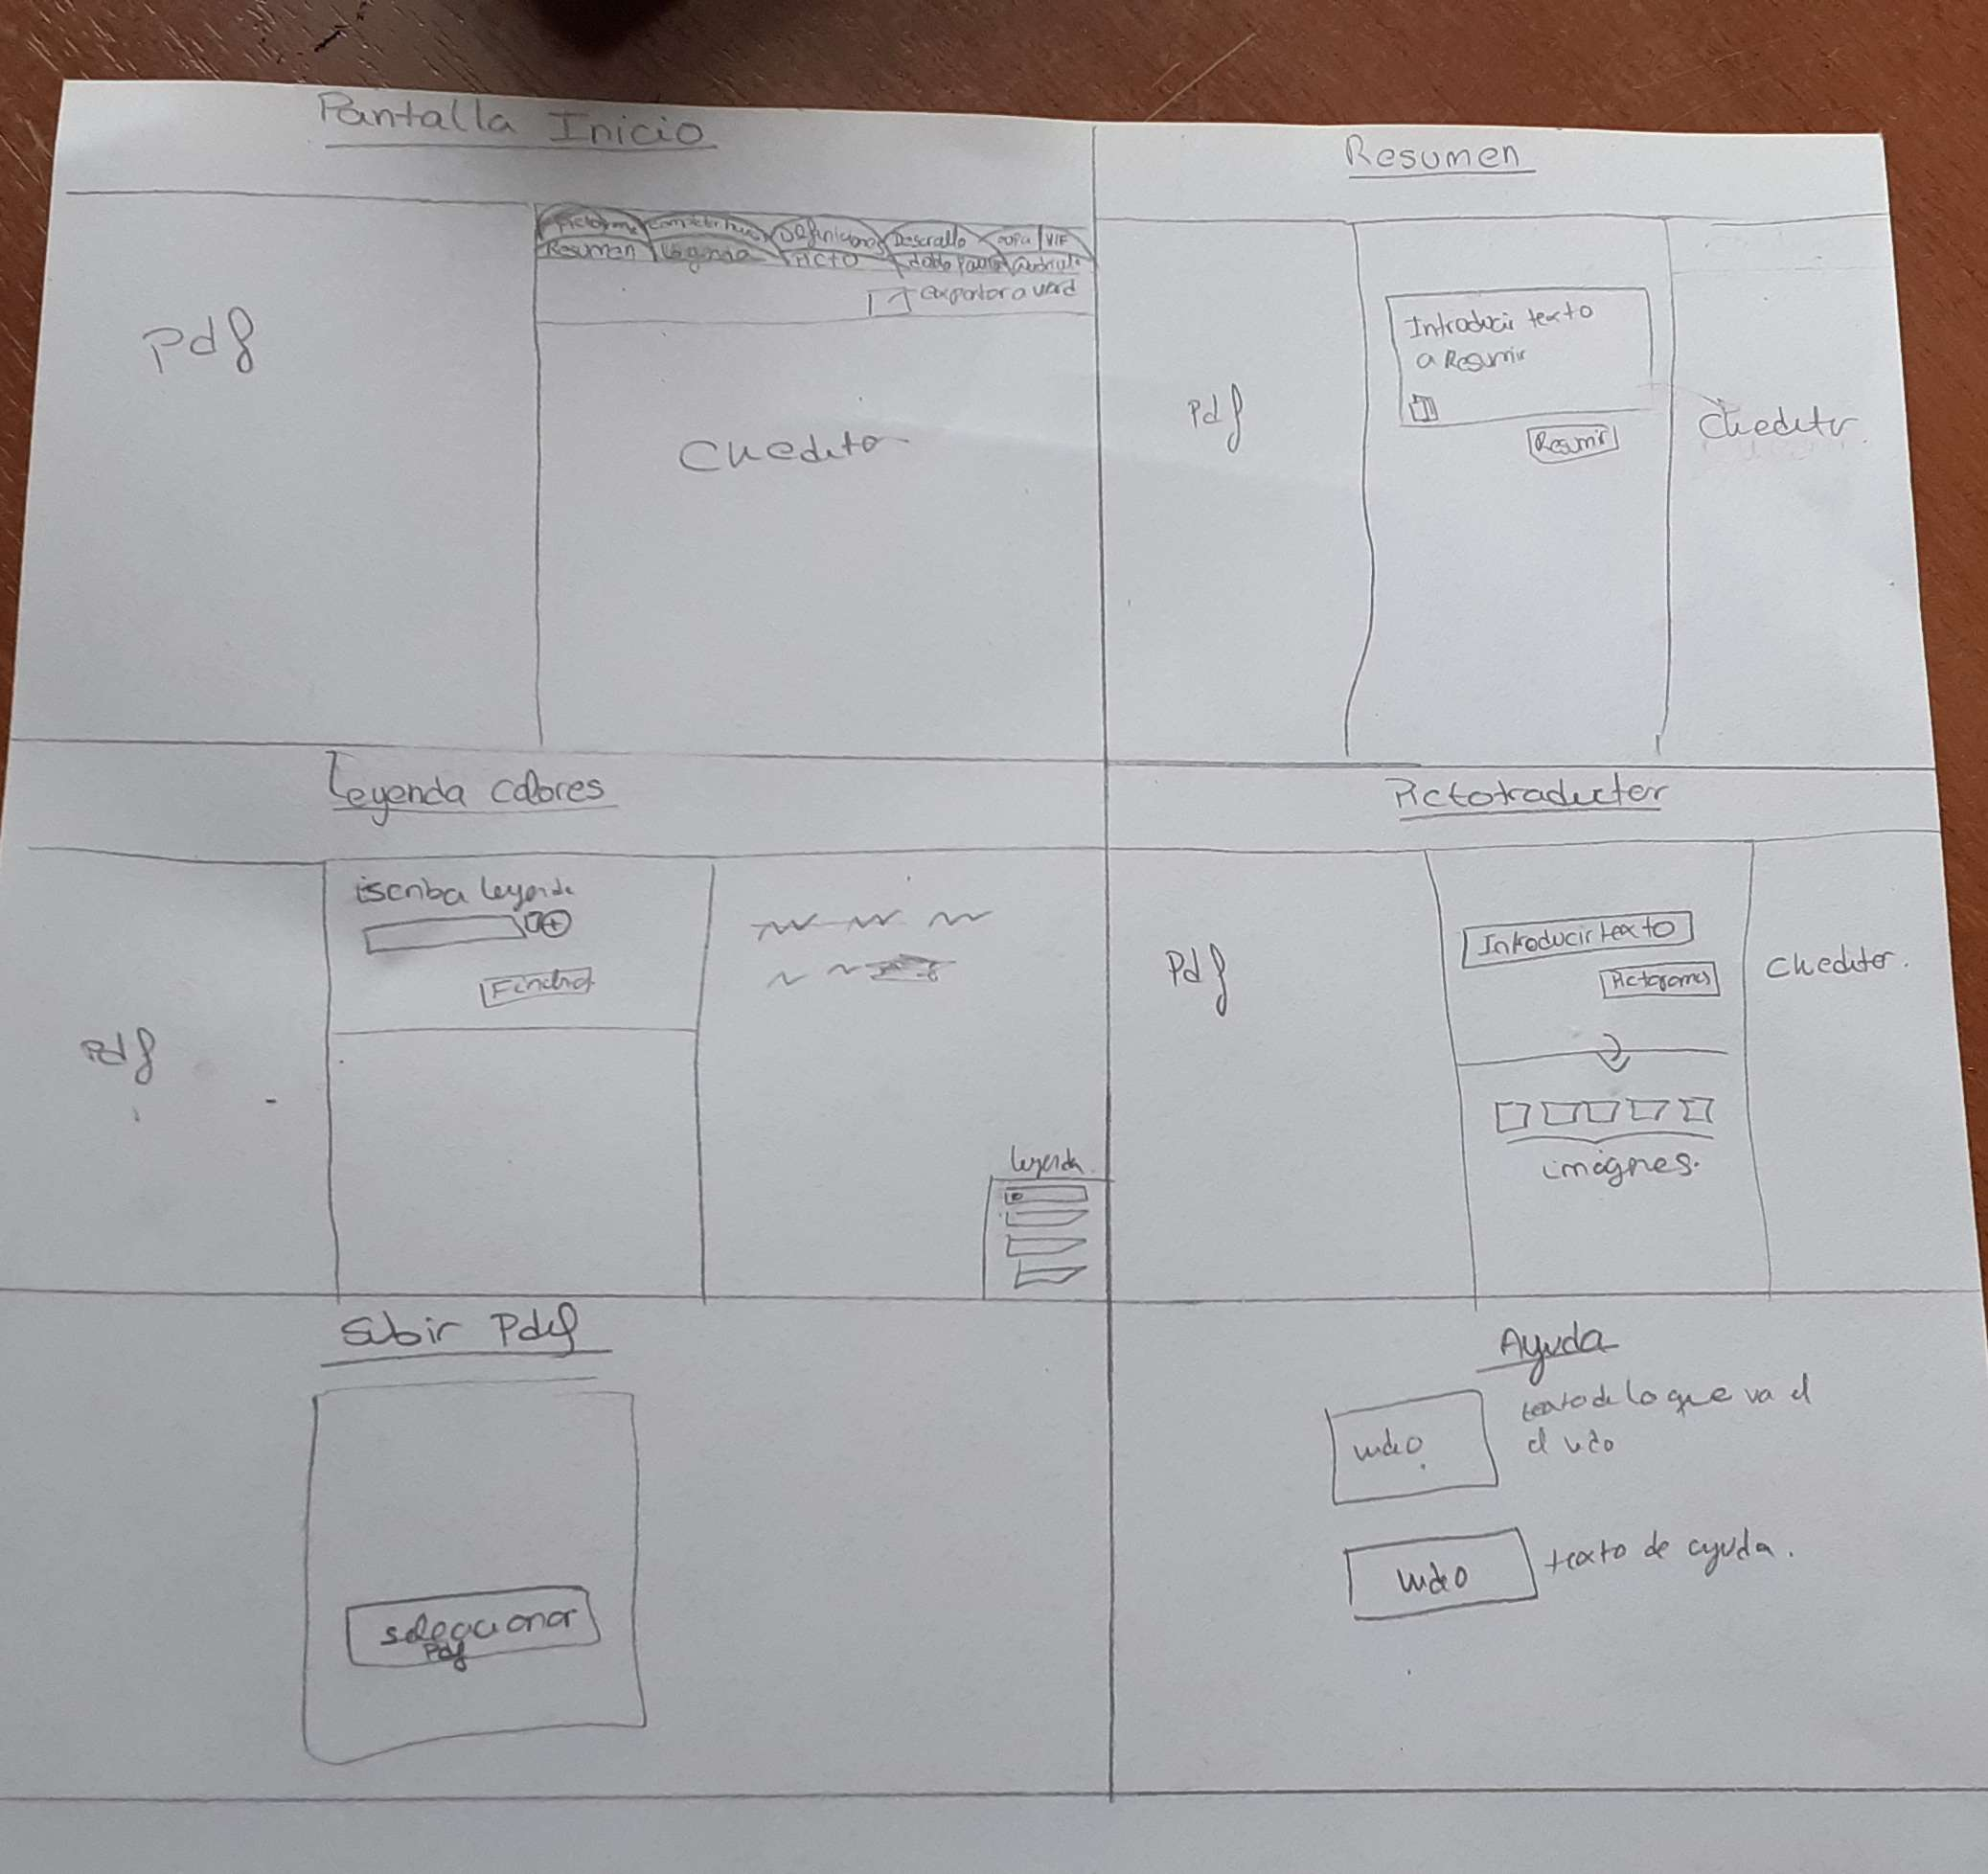
\includegraphics[width=15cm]{Diseño/Dunia.jpg}
    \caption{Diseño Dunia Namour Doughani iteración competitiva .}
    \label{IteracionCompetitiva3}
\end{figure}
\begin{figure}[ht!]
    \centering
    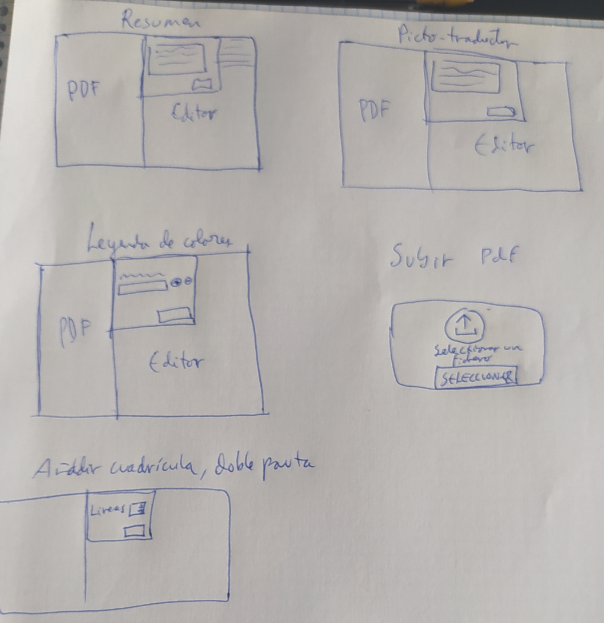
\includegraphics[width=15cm]{Diseño/Alberto.jpg}
    \caption{Diseño 1 Alberto Alejandro Rivas Fernández iteración competitiva.}
    \label{IteracionCompetitiva4}
\end{figure}
\begin{figure}[ht!]
  \centering
  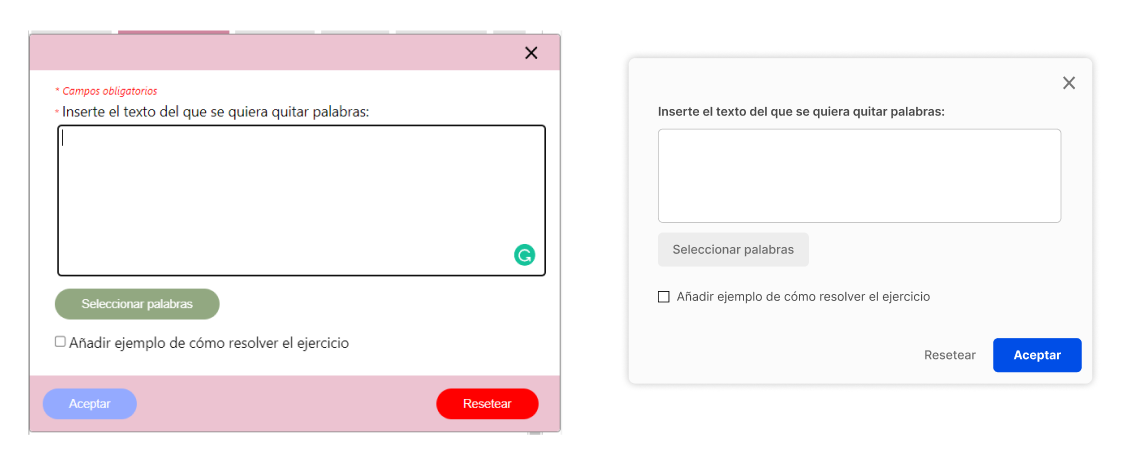
\includegraphics[width=13cm]{Diseño/Alberto2.png}
  \caption{Diseño 2 Alberto Alejandro Rivas Fernández iteración competitiva.}
  \label{IteracionCompetitivaA2}
\end{figure}
\begin{figure}[ht!]
  \centering
  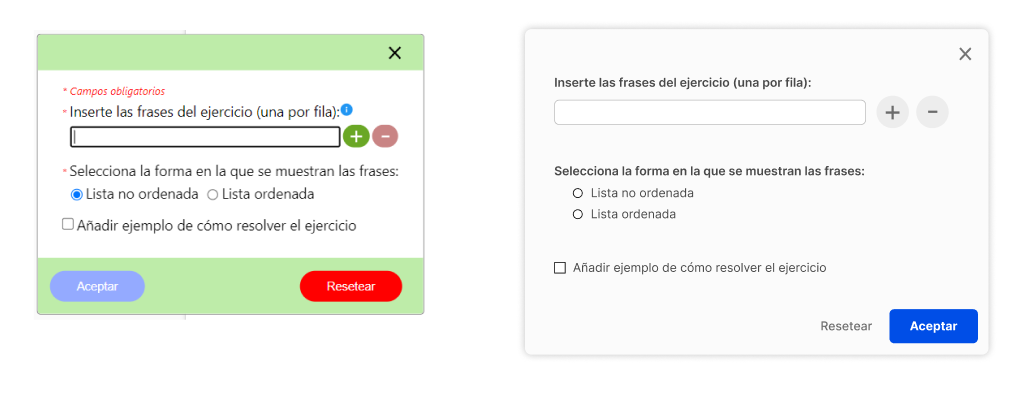
\includegraphics[width=13cm]{Diseño/Alberto4.png}
  \caption{Diseño 3 Alberto Alejandro Rivas Fernández iteración competitiva.}
  \label{IteracionCompetitivaA3}
\end{figure}
\begin{figure}[ht!]
  \centering
  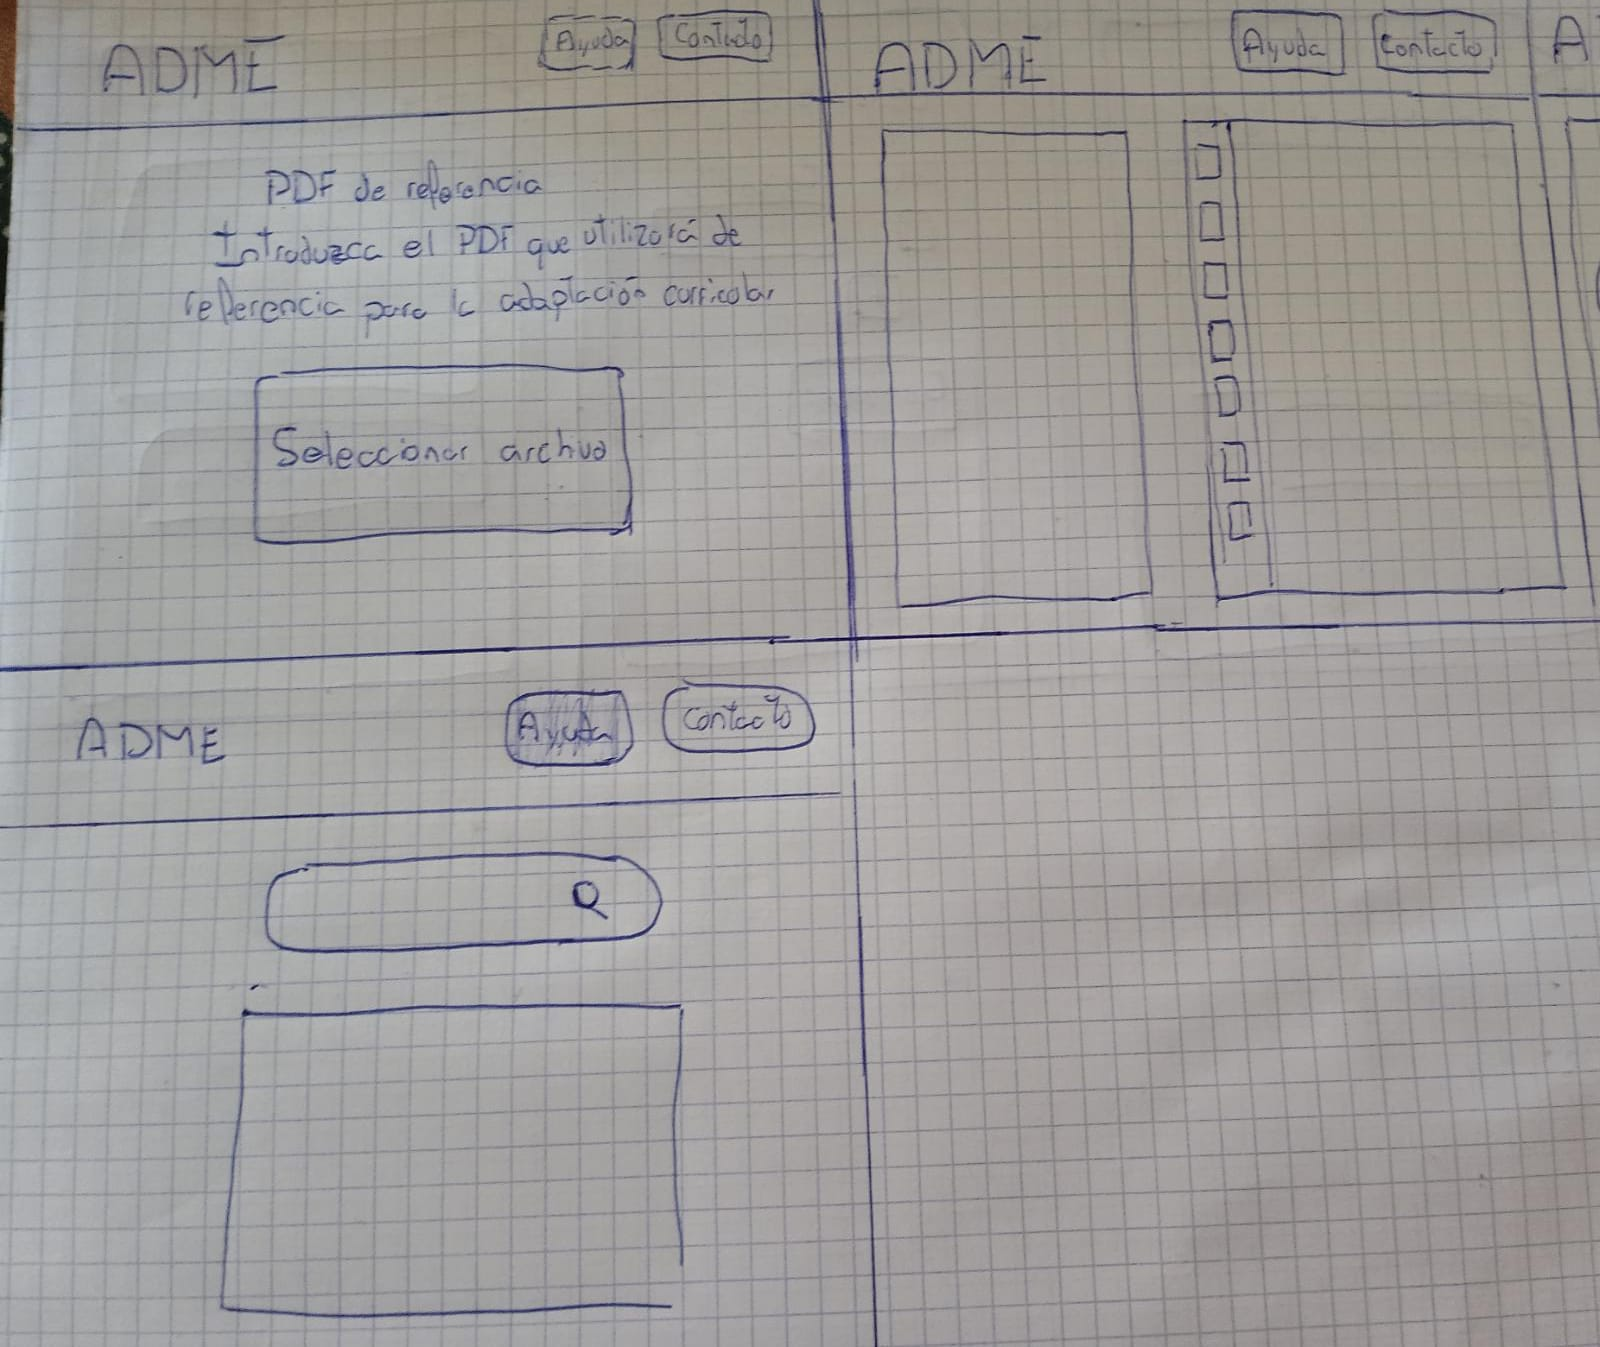
\includegraphics[width=15cm]{Diseño/Johan.jpeg}
  \caption{Diseño 3 Johan Sebastian Salvatierra Gutierrez iteración competitiva.}
  \label{IteracionCompetitivaJ1}
\end{figure}
\begin{figure}[ht!]
  \centering
  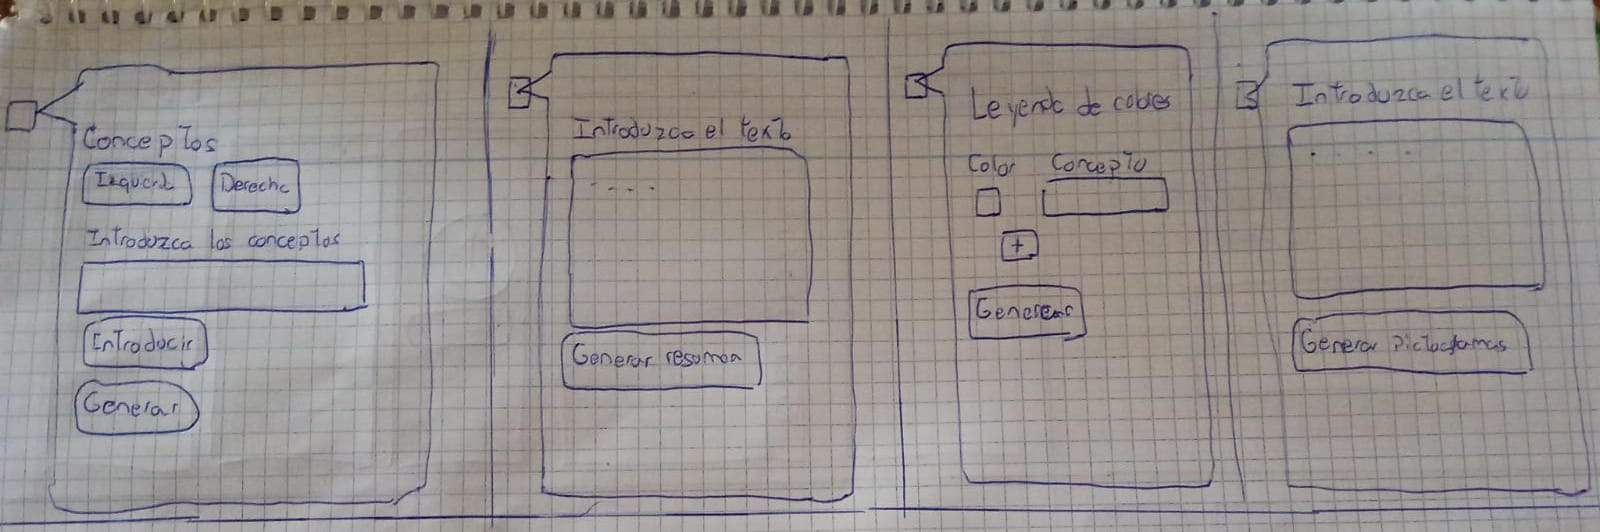
\includegraphics[width=15cm]{Diseño/Johan2.jpeg}
  \caption{Diseño 3 Johan Sebastian Salvatierra Gutierrez iteración competitiva.}
  \label{IteracionCompetitivaJ2}
\end{figure}
\begin{figure}[ht!]
  \centering
  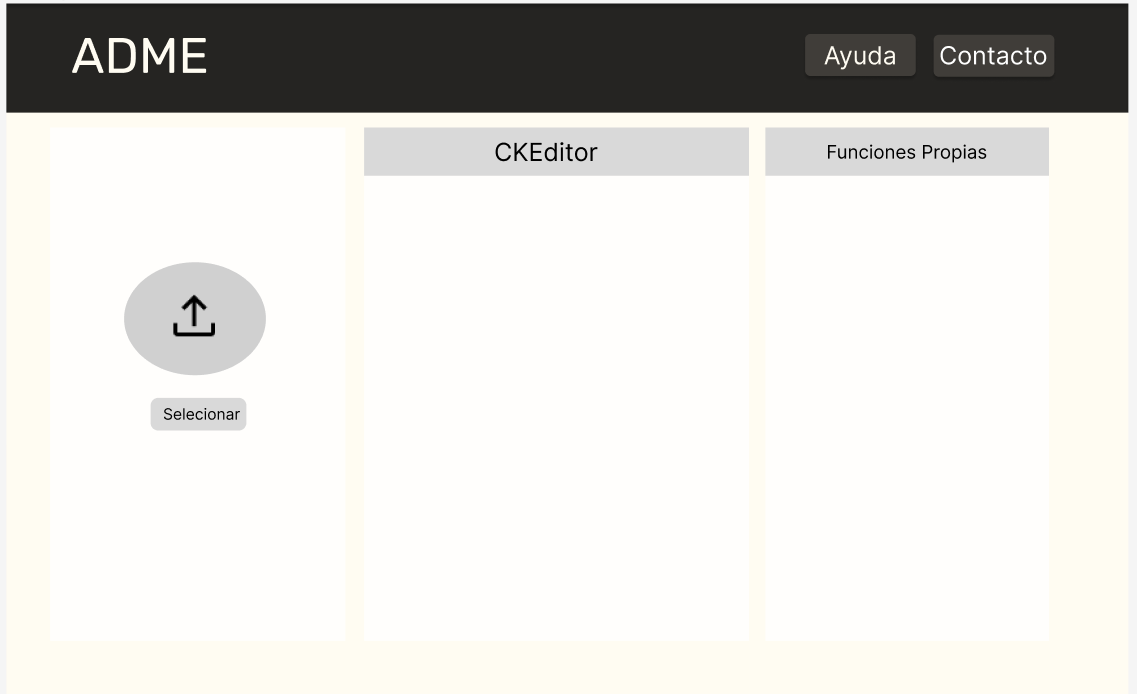
\includegraphics[width=10cm]{Diseño/Diseño Final}
  \caption{Diseño pantalla de inicio.}
  \label{diseño_final}
\end{figure}
\begin{figure}[ht!]
  \centering
  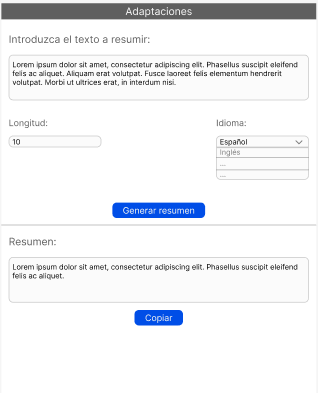
\includegraphics[width=10cm]{Diseño/resumen}
  \caption{Diseño funcionalidad generar un resumen a partir de un texto.}
  \label{resuemn}
\end{figure}
\begin{figure}[ht!]
  \centering
  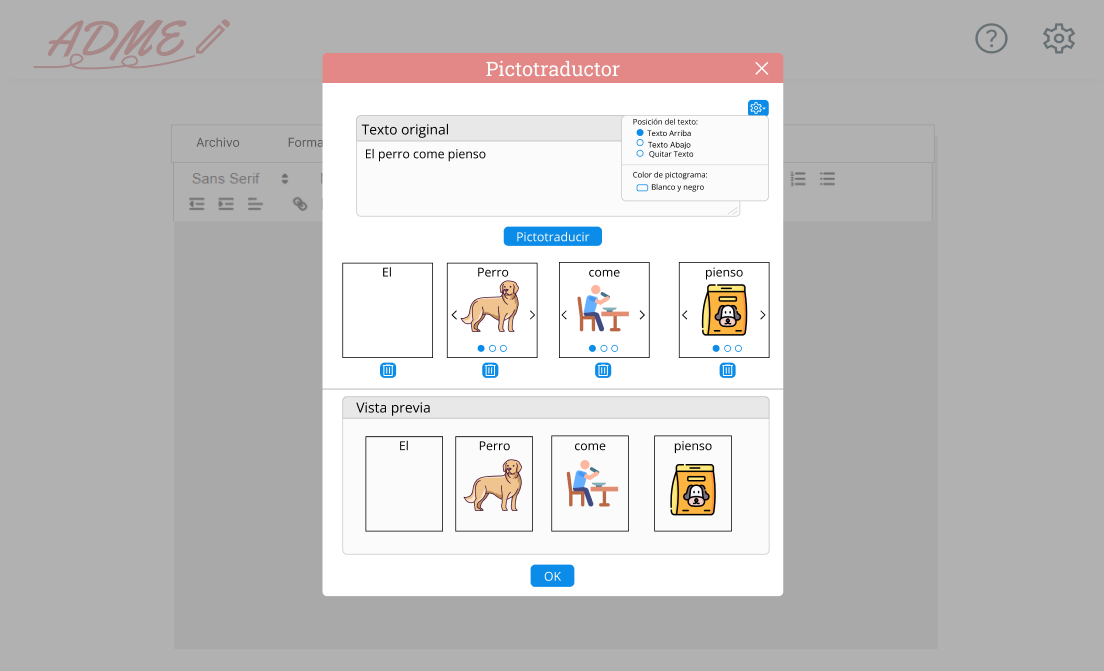
\includegraphics[width=10cm]{Diseño/picto}
  \caption{Diseño funcionalidad añadir pictotraductor.}
  \label{picto}
\end{figure}
\begin{figure}[ht!]
  \centering
  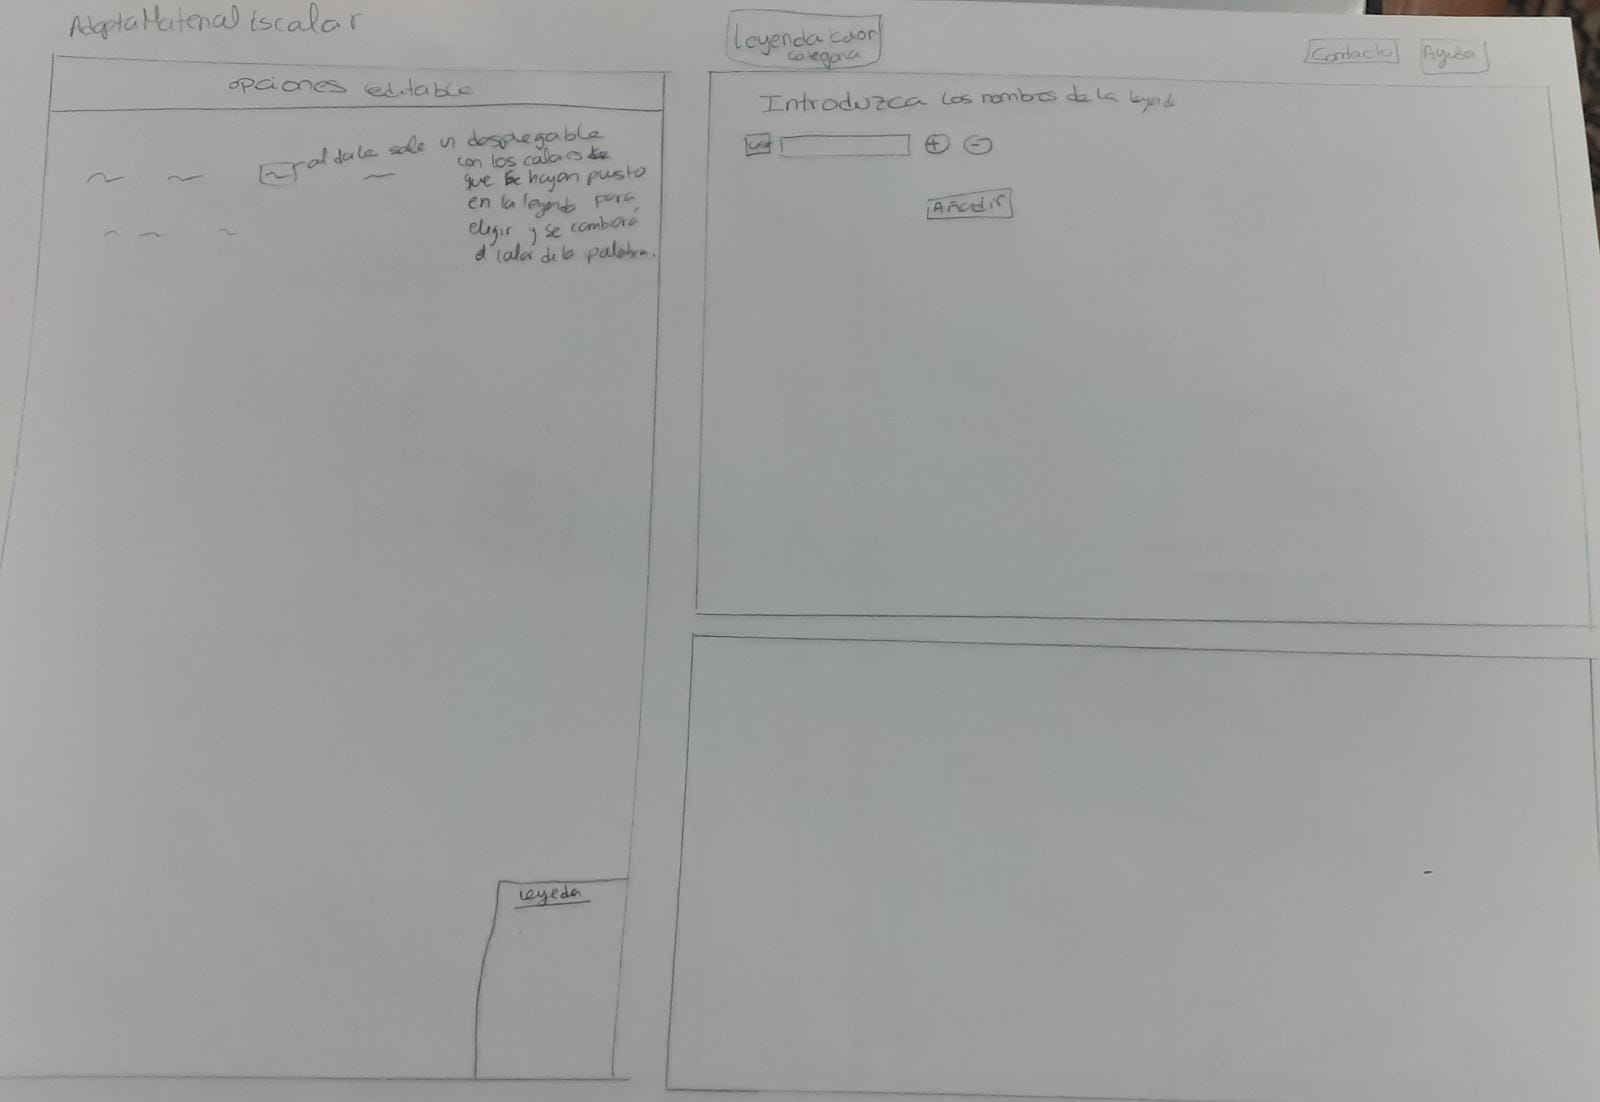
\includegraphics[width=10cm]{Diseño/leyendaColor}
  \caption{Diseño funcionalidad añadir una leyenda de colores con la categoría de cada tipo.}
  \label{leyenda}
\end{figure}
\begin{figure}[ht!]
  \centering
  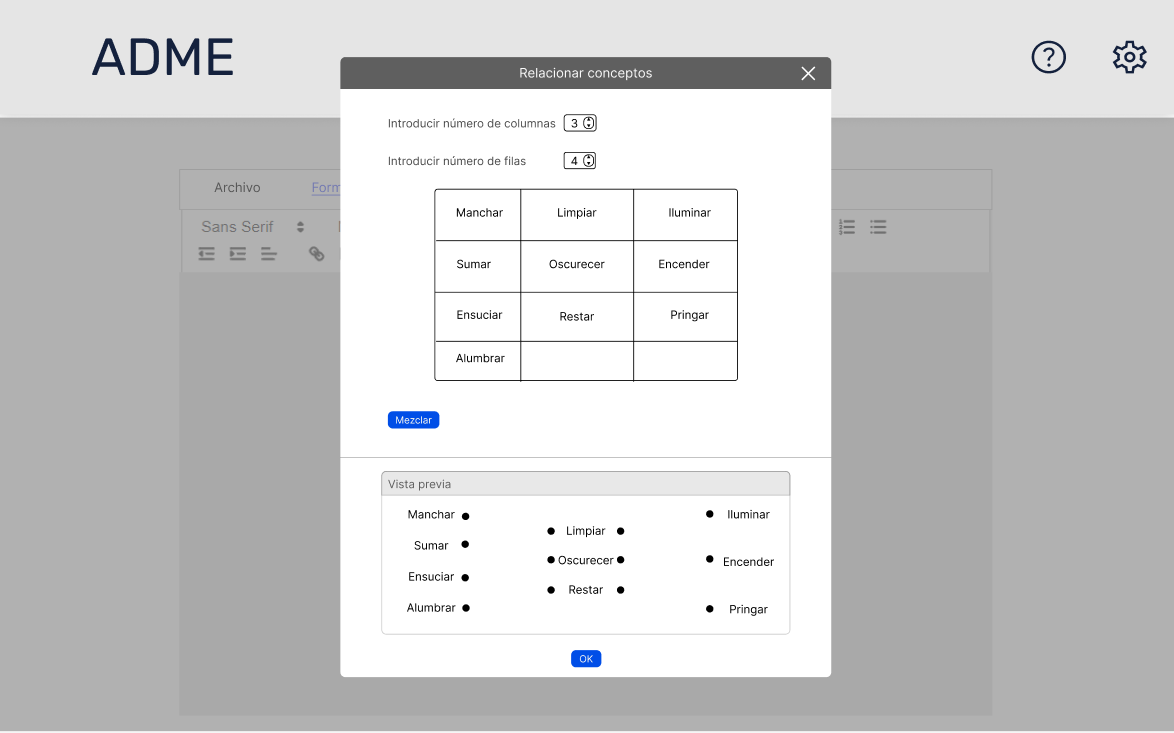
\includegraphics[width=10cm]{Diseño/flechas}
  \caption{Diseño funcionalidad ejercicios de relacionar contenido mediante flechas.}
  \label{flecha}
\end{figure}